\chapter{Evoluindo uma plataforma de rede social}
\label{evol-rede-social}
%
\section{Noosfero}
\label{evol-rede-social}

O Noosfero \footnote{\url{http://www.noosfero.org}} é uma plataforma de criação de redes sociais livre desenvolvida em 2007 pela Cooperativa de Tecnologias Livres - Colivre \footnote{\url{http://www.colivre.coop.br}}, sob a licença AGPL\footnote{Licença de software GNU Affero General Public License} V3, com a proposta de facilitar a criação de redes sociais personalizadas, livres e autônomas e a geração de conteúdo colaborativo.

A Colivre é uma cooperativa sediada em Salvador/BA e trabalha contribuindo  com a difusão e o desenvolvimento de tecnologias livres. Atualmente os desenvolvedores da Colivre realizam a manutenção e evolução do Noosfero além de manter seu repositório, ou seja, são responsáveis por revisar os códigos que são enviados pela comunidade e integrar ao código do Noosfero.

Além das funcionalidades de rede social, com foco na produção e compartilhamento de
conteúdo, o Noosfero permite que dentro da rede cada usuário e comunidade tenha o seu espaço com total flexibilidade de personalização visual e gerenciamento de conteúdo. A exemplo de portais que atualmente utilizam o Noosfero temos o Participa BR \footnote{\url{https://www.participa.br/}}, o Stoa\footnote{\url{http://stoa.usp.br/}} e o Portal da FGA\footnote{\url{http://fga.unb.br/}}.

O Noosfero foi desenvolvido na linguagem de programação Ruby, atualmente na versão 2.2.0, e utiliza o \textit{framework} aplicações web \textit{Ruby on Rails} \footnote{\url{http://rubyonrails.org/}}, versão 3.2.21. E utiliza também padrões arquiteturais de software Model-View-Controller (MVC), e o padrão de plugins que serão apresentados na seção \ref{arquitetura}.

A escolha da linguagem \textit{Ruby} foi decisiva no Noosfero, pois possui uma sintaxe simples, que facilita a manutenibilidade do sistema, característica importante em projetos de software livre que tendem a atrair colaboradores externos a equipe \cite{meirelles2013}. A escolha do \textit{Rails} foi influenciada pelos seus conceitos básicos de existência que auxiliam em sua produtividade, são estes, o "Não Repita a Si Mesmo" (DRY-\textit{Don't Repeat Yourself}) e "convenção sobre configuração" (\textit{convention over configuration}) \cite{akita2006repensando}.

Por questões de segurança o Noosfero utiliza apenas pacotes os pacotes \textit{stable} do \textit{Debian}, por serem reconhecidas por sua estabilidade e testes de segurança antes de seu lançamento, atualmente compreende a versão \textit{Wheezy}. Além de utilizar o pacote do \textit{Ruby on Rails} oficial do \textit{Debian}, de forma que uma vez que a vulnerabilidade é corrigida no Debian, não é preciso corrigir no Noosfero.

\subsection{Software Livre}
\label{soft-livre}

De acordo com \cite{meirelles2013} software expressa uma solução abstrata dos problemas computacionais, neste contexto é o componente que contém o conhecimento relacionado aos problemas a que a computação se aplica, contendo diversos aspectos que ultrapassam questões técnicas, a exemplo temos:
\begin{itemize}
\item O processo de desenvolvimento do software;
\item Os mecanismos econômicos (gerenciais, competitivos, sociais, cognitivos etc.) que regem esse desenvolvimento e seu uso;
\item O relacionamento entre desenvolvedores, fornecedores e usuários do software;
\item Os aspectos éticos e legais relacionados ao software
\end{itemize}

O que define e diferencia o software livre de software proprietário vai do entendimento desses quatro pontos dentro do que é conhecido como \textit{ecossistema do software livre}~\cite{meirelles2013}.

Software livre é definido pela Free Software Foundation como “uma questão de liberdade dos usuários para executar, copiar, distribuir, estudar, mudar e melhorar o software. Levando isto em consideração significa que os usuários do software possuem quatro liberdades essenciais \cite{stallman2002free}:

\begin{itemize}
\item A liberdade de executar o programa, para qualquer propósito (liberdade no. 0);
\item A liberdade de estudar como o programa funciona, e adaptá-lo para as suas necessidades (liberdade no. 1). Aceso ao código-fonte é um pré-requisito para esta liberdade;
\item A liberdade de redistribuir cópias de modo que você possa ajudar ao seu próximo (liberdade no. 2);
\item A liberdade de aperfeiçoar o programa, e liberar os seus aperfeiçoamentos, de modo que toda a comunidade se beneficie (liberdade no. 3). Acesso ao código-fonte é um pré-requisito para esta liberdade.
\end{itemize}

Para que as liberdades um e três façam sentido, é necessário que o desenvolvedor ou pesquisador tenha acesso ao código-fonte do programa.  Portanto, acesso ao código-fonte é uma condição necessária ao software livre ~\cite{gnu2013}.

Um programa é considerado um software livre se os usuários possuem todas as liberdades citadas. Dessa forma, você deve ser livre para redistribuir cópias, com ou sem modificações, de graça ou cobrando uma taxa pela distribuição, para qualquer lugar. Ser livre para fazer essas coisas significa (entre outras coisas) que você não tem que pedir ou pagar por permissão para fazê-las ~\cite{anaPaula2012}.

O fato de que o código-fonte pode ser livremente compartilhado oferece vantagens ao software livre em comparação ao software proprietário. Umas delas é que podem simplificar o desenvolvimento de aplicações personalizadas já que não precisam ser programadas a partir do zero podem se basear em soluções já existentes.

A outra vantagem resultante do compartilhamento do código refere-se à possível melhoria na qualidade, em particular frente aos problemas inerentes à sua complexidade \cite{catedralBazzar}.
%
Isso se deve ao maior número de desenvolvedores e usuários envolvidos com o software, permitindo maiores situações de uso e necessidades mais variadas, o que propicia a identificação de um número maior de \emph{bugs} e mais sugestões de melhoria, promovendo refatorações que geralmente levam a melhoria do código.

O GNU quis dar aos utilizadores a liberdade, não só para ser popular. Contudo precisava usar termos de distribuição que impediriam software livre de ser transformado em software proprietário. O método usado foi chamado de \emph{copyleft}. \emph{Copyleft} é um método geral para fazer um software livre e exige que todas as versões modificadas e estendidas do programa sejam também. Ele utiliza lei de direitos autorais, mas veio para servir como oposto de sua finalidade usual: ao invés de um meio de privatizar o software, torna-se um meio de manter o software livre~\cite{stallman2009}.

\subsection{Processos e desenvolvimento da comunidade}
\label{proc-desenvol-comunidade}
% - ciclos
% - repositorio
% - commiters/revisao
% - testes

Para que novos desenvolvedores colaborem com o Noosfero a comunidade utiliza em seu próprio \textit{site} uma seção para o desenvolvimento. Nesta seção tem-se manuais com os passos para instalação do ambiente, descrição dos \textit{plugins} disponíveis, instruções para a personalização da plataforma através de temas além de informações arquiteturais para os colaboradores com a plataforma. Para realizar o controle de itens a fazer como a implementação de novas funcionalidaes ou correção de bugs é utilizado um \textit{Issue Tracker}.

Uma vez que o desenvolvedor tenha registro no site da comunidade é possível utilizar o \textit{Issue Tracker} para cadastrar novas funcionalidades \textit{new features} ou \textit{bugs} de maneira simples conforme os seguintes passos:

\begin{enumerate}
\item Preencher o campo título;
\item Definir a quais categorias o item pertence (e.g. Chat, RSSFeeds);
\item Definir a descrição do item;
\item Especificar com qual \textit{plugin} o item está relacionado (se existir);
\item Especificar qual a versão do Noosfero o item afeta.
\end{enumerate}

Com algumas ressalvas que para funcionalidades, coloca-se a versão em que essa está prevista para ser lançada, enquanto que para bugs, coloca-se também a versão em que este foi identificado. Com o item criado, outros usuários podem adicionar comentários e associar um desenvolvedor responsável pela sua implementação.

A figura \ref{issue-tracker} evidencia o \textit{Issue Treacker} do Noosfero onde é possível verificar os itens que foram mapeados e seus respectivos \textit{status} (concluído, pendente, rejeitado, trabalhando, esperando FeedBack). Dessa forma, é possível priorizar os itens identificados como sendo de maior importância para os usuários e desenvolvedores

\begin{figure}[h]
    \centering
    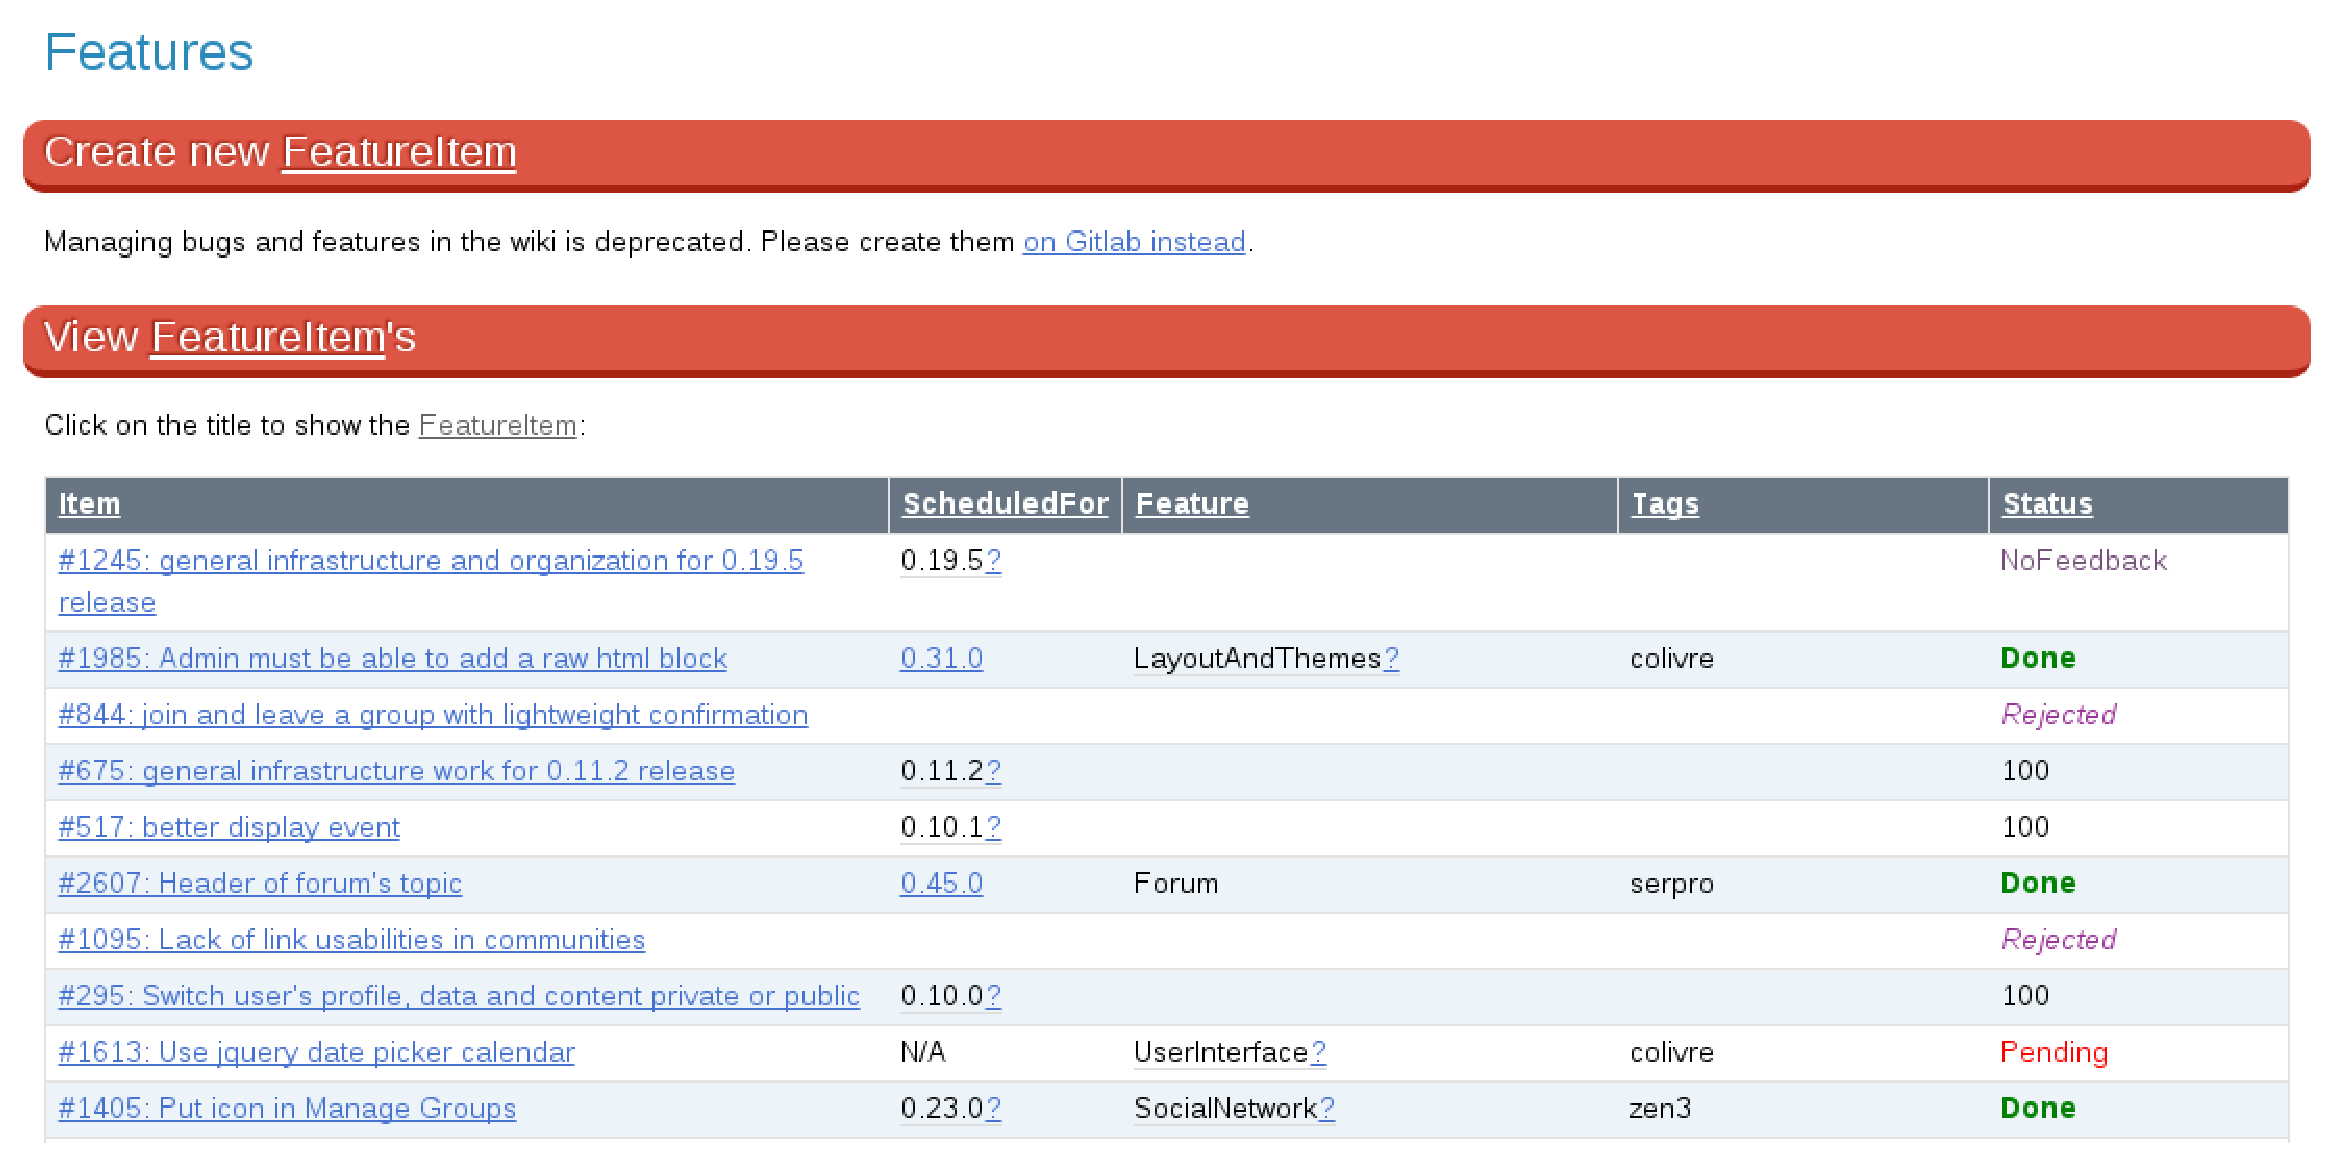
\includegraphics[keepaspectratio=true,scale=0.4]
      {figuras/issueTrackerNoosfero.eps}
    \caption{Issue Tracker no site do Noosfero}
    \label{issue-tracker}
\end{figure}

A implementação é realizada pelo desenvolvedor que tem a responsabilidade de manter a qualidade do código produzido bem como todos os testes relacionados à funcionalidade implementada. Uma vez que este primeiro passo esteja concluído o código é submetido a um \textit{merge-request} onde algum dos desenvolvedores do \textit{core} revisa para verificar se está de acordo com os padrões esperados, e aprova ou não, a inclusão do código na \textit{branch} principal do Noosfero.

A comunidade Noosfero adota e recomenda práticas de desenvolvimento como o TDD, \textit{Test Driven Development} ou Desenvolvimento orientado a testes), combinado com o BDD \footnote{\url{https://cukes.info/}} (\textit{Behavior Driven Development}ou Desenvolvimento Guiado por Comportamento, que possibilita o desenvolviemnto de um código tenha uma maior coesão e um menor acoplamento.

Para realizar o controle de versão e gerenciamento do código fonte é utilizado o Git, uma ferramenta livre de versionamento distribuído de código fonte. O repositório oficial do Noosfero encontra-se no software livre Gitlab\footnote{\url{https://gitlab.com/noosfero/noosfero}} com um espelho no Github\footnote{\url{https://github.com/noosfero/noosfero}}. Na página de desenvolvimento da comunidade existe uma série de recomendações sobre como enviar patches para o Noosfero, desde como versionar seu patches, até como realizar a solicitação de inclusão do seu patch, ou \textit{merge-request}, na plataforma.

\subsection{Arquitetura}
\label{arquitetura}

- plugins

Como um software está em constante evolução a arquitetura do Noosfero foi criada para ser altamente expansível fazendo-se o uso de \textit{plugins}. Essa arquitetura permite que em cada ambiente fique a critério do usuário quais os \textit{plugins}, novas funcionalidades, serão habilitadas o que torna o sistema flexível e modular.

Essa arquitetura extensível adotada pelo Noosfero auxilia no controle da qualidade de código das novas funcionalidades. Os mesmos são mantidos em uma pasta \textit{plugins} fora do escopo do código  do núcleo do software, ou seja, o desenvolvedor cria novas funcionalidades sem modificar o \textit{core} do Noosfero.

Um programa que utiliza o paradigma orientado a eventos não controla a sequência na qual ocorrem os eventos de entrada ele apenas reagem a uma sequência razoável de eventos \cite{tucker2009linguagens}. O funcionamento dos plugins do Noosfero é baseado neste paradigma, onde o o núcleo do Noosfero dispara um evento durante a execução de alguma funcionalidade, e os \textit{plugins} interessados nesse evento são capazes de executar suas ações tratando o evento de acordo com sua implementação. No Noosfero os eventos são conhecidos como "\textit{hotspots}".

Como mencionado na seção \ref{proc-desenvol-comunidade} o Noosfero faz uso de testes para manter a integridade de seu cógido, dessa maneira também é necessário que os \textit{plugins} contenham seus respectivos testes para evitar a inserção de \textit{bugs} e mudanças inesperadas no comportamento do sistema.

\subsection{Comunidade UnB}
\label{comunidade-unb}
- funcionalidades

\section{Desenvolvimento do NoosferAVA}
\label{desen-noosferAVA}
- requisitos
-- funcionalidades adaptadas/melhoras
-- novas funcionalidades

-Atualizar pro rails 3

-Utilização do LDAP
	-realizar melhorias
		-cadastro de matricula dos usuários já existentes
		-

-Evolução do workassigment
	-permitir atribuição de notas para a atividade
	-**timer (plugin de tolerância e tempo)

-*Calendário de atividades
	-Arquivos do work assigment

-Definir template de disciplina

-Sistema de notas